\subsection{Question 1.1}

Tina nous donne le p-flot suivant pour le premier schéma :\\

\begin{center}

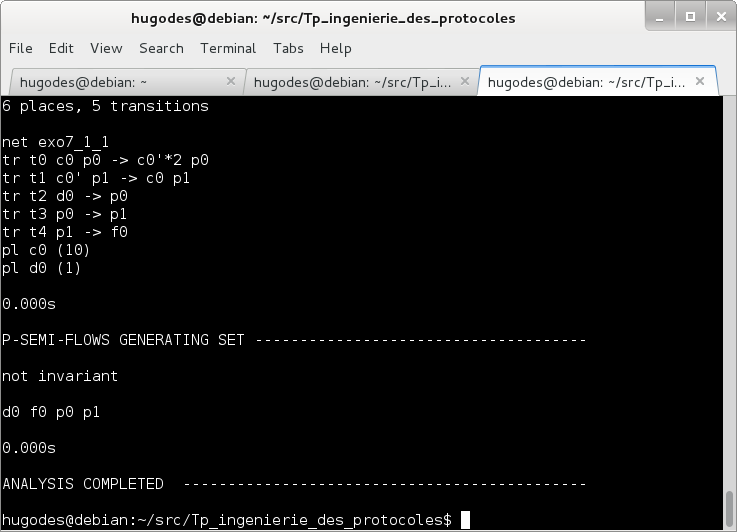
\includegraphics[width=0.7\textwidth]{exo7/tina_7_1.png}\\

\end{center}

On va utiliser l'algorithme de Farkas pour calculer les P-semi flots du premier schéma.

\begin{center}

{\Huge C}\qquad =\qquad $\bordermatrix{
&t_1&t_2&t_3&t_4&t_5\cr
d0&-1&0&0&0&0\cr
p0&1&-1&0&0&0\cr
p1&0&1&-1&0&0\cr
f0&0&0&1&0&0\cr
c0&0&0&0&-1&1\cr
c'0&0&0&0&2&-1\cr
}$

{\Huge $\downarrow$}

$\bordermatrix{
&t_2&t_3&t_4&t_5\cr
d0+p0&-1&0&0&0\cr
p1&1&-1&0&0\cr
f0&0&1&0&0\cr
c0&0&0&-1&1\cr
c'0&0&0&2&-1\cr
}$

{\Huge $\downarrow$}

$\bordermatrix{
&t_3&t_4&t_5\cr
d0+p0+p1&-1&0&0\cr
f0&1&0&0\cr
c0&0&-1&1\cr
c'0&0&2&-1\cr
}$

{\Huge $\downarrow$}

$\bordermatrix{
&t_4&t_5\cr
d0+p0+p1+f0&0&0\cr
c0&-1&1\cr
c'0&2&-1\cr
}$


\vspace{1cm}

On trouve donc un P-semi flot :\\
$f_2 = (1\ 1\ 1\ 1\ 0\ 0)$

On obtient donc le même résultat que TINA.

\end{center}


\subsection{Question 1.2}
Tina nous donne le p-flot suivant pour le second schéma :\\

\begin{center}

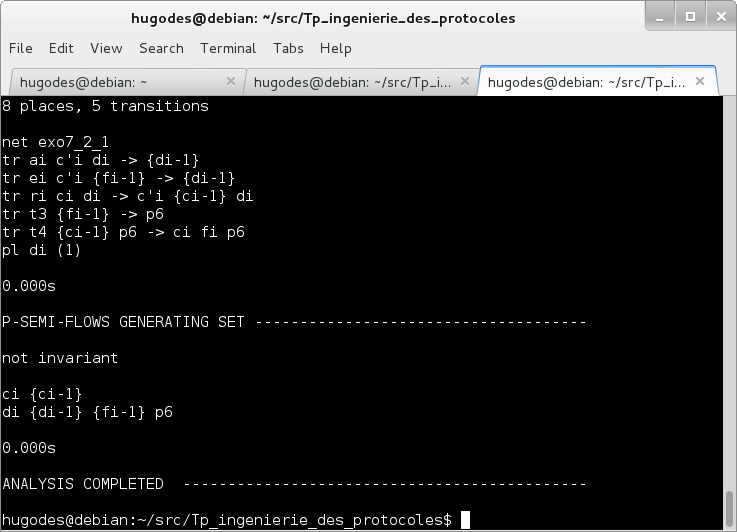
\includegraphics[width=0.7\textwidth]{exo7/tina_7_2.png}\\

\end{center}

On va utiliser l'algorithme de Farkas pour calculer les P-semi flots du second schéma.

\begin{center}


{\Huge C}\qquad =\qquad $\bordermatrix{
&ai&ei&ri&t1&t2\cr
ci&0&0&-1&0&1\cr
c'i&-1&-1&1&0&0\cr
ci-1&0&0&1&0&-1\cr
di&-1&0&0&0&0\cr
di-1&1&1&0&0&0\cr
fi-1&0&-1&0&-1&0\cr
fi&0&0&0&0&1\cr
p1&0&0&0&1&0\cr
}$

{\Huge $\downarrow$}

$\bordermatrix{
&ei&ri&t1&t2\cr
ci&0&-1&0&1\cr
c'i+di-1&0&1&0&0\cr
ci-1&0&1&0&-1\cr
di+di-1&1&0&0&0\cr
fi-1&-1&0&-1&0\cr
fi&0&0&0&1\cr
p1&0&0&1&0\cr
}$

{\Huge $\downarrow$}

$\bordermatrix{
&ri&t1&t2\cr
ci&-1&0&1\cr
c'i+di-1&1&0&0\cr
ci-1&1&0&-1\cr
di+di-1+fi-1&0&-1&0\cr
fi&0&0&1\cr
p1&0&1&0\cr
}$

{\Huge $\downarrow$}

$\bordermatrix{
&t1&t2\cr
c'i+di-1+ci&0&1\cr
ci-1+ci&0&0\cr
di+di-1+fi-1&-1&0\cr
fi&0&1\cr
p1&1&0\cr
}$

{\Huge $\downarrow$}

$\bordermatrix{
&t2\cr
c'i+di-1+ci&1\cr
di+di-1+fi-1+p1&0\cr
fi&1\cr
}$

\vspace{1cm}

On trouve donc 2 P-semi flots :\\
$f_1 = (0\ 1\ 1\ 0\ 0\ 0\ 0\ 0)$\\
$f_2 = (0\ 0\ 1\ 1\ 1\ 0\ 0\ 1)$\\

\end{center}

On obtient donc le même résultat que TINA.


\subsection{Question 2.1}
Pour le premier schéma la séquence maximale est:\\
t1 -> n*t4 -> t2 -> 2n*t5 -> t3 

\subsection{Question 2.2}
Pour le second schéma la séquence maximale est:\\
t1 -> n*t4 -> t2 -> 2n*t5 -> t3 